\documentclass[14pt]{extbook}
\usepackage{multicol, enumerate, enumitem, hyperref, color, soul, setspace, parskip, fancyhdr} %General Packages
\usepackage{amssymb, amsthm, amsmath, bbm, latexsym, units, mathtools} %Math Packages
\everymath{\displaystyle} %All math in Display Style
% Packages with additional options
\usepackage[headsep=0.5cm,headheight=12pt, left=1 in,right= 1 in,top= 1 in,bottom= 1 in]{geometry}
\usepackage[usenames,dvipsnames]{xcolor}
\usepackage{dashrule}  % Package to use the command below to create lines between items
\newcommand{\litem}[1]{\item#1\hspace*{-1cm}\rule{\textwidth}{0.4pt}}
\pagestyle{fancy}
\lhead{Progress Quiz 9}
\chead{}
\rhead{Version C}
\lfoot{8590-6105}
\cfoot{}
\rfoot{Fall 2020}
\begin{document}

\begin{enumerate}
\litem{
Solve the rational equation below. Then, choose the interval(s) that the solution(s) belongs to.\[ \frac{5x}{4x + 3} + \frac{-4x^{2}}{16x^{2} -8 x -15} = \frac{3}{4x -5} \]\begin{enumerate}[label=\Alph*.]
\item \( x_1 \in [-2.7, 0.4] \text{ and } x_2 \in [-0.4,6] \)
\item \( \text{All solutions lead to invalid or complex values in the equation.} \)
\item \( x_1 \in [-2.7, 0.4] \text{ and } x_2 \in [-1.8,-0.6] \)
\item \( x \in [0.4,2] \)
\item \( x \in [1.9,4.7] \)

\end{enumerate} }
\litem{
Determine the domain of the function below.\[ f(x) = \frac{5}{30x^{2} -49 x + 20} \]\begin{enumerate}[label=\Alph*.]
\item \( \text{All Real numbers except } x = a, \text{ where } a \in [19.98, 20.01] \)
\item \( \text{All Real numbers except } x = a \text{ and } x = b, \text{ where } a \in [0.77, 0.83] \text{ and } b \in [0.82, 0.86] \)
\item \( \text{All Real numbers except } x = a \text{ and } x = b, \text{ where } a \in [19.98, 20.01] \text{ and } b \in [29.97, 30.02] \)
\item \( \text{All Real numbers except } x = a, \text{ where } a \in [0.77, 0.83] \)
\item \( \text{All Real numbers.} \)

\end{enumerate} }
\litem{
Solve the rational equation below. Then, choose the interval(s) that the solution(s) belongs to.\[ \frac{-60}{60x + 30} + 1 = \frac{-60}{60x + 30} \]\begin{enumerate}[label=\Alph*.]
\item \( x_1 \in [-2.7, -0.4] \text{ and } x_2 \in [-0.3,1.4] \)
\item \( \text{All solutions lead to invalid or complex values in the equation.} \)
\item \( x \in [-2.5,0.5] \)
\item \( x_1 \in [-2.7, -0.4] \text{ and } x_2 \in [-1.5,0] \)
\item \( x \in [-0.2,0.8] \)

\end{enumerate} }
\litem{
Solve the rational equation below. Then, choose the interval(s) that the solution(s) belongs to.\[ \frac{24}{48x -36} + 1 = \frac{24}{48x -36} \]\begin{enumerate}[label=\Alph*.]
\item \( x \in [-0.25,2.75] \)
\item \( x \in [-0.75,0.25] \)
\item \( x_1 \in [0.75, 2.75] \text{ and } x_2 \in [-0.25,1.75] \)
\item \( x_1 \in [-0.75, 0.25] \text{ and } x_2 \in [-0.25,1.75] \)
\item \( \text{All solutions lead to invalid or complex values in the equation.} \)

\end{enumerate} }
\litem{
Choose the graph of the equation below.\[ f(x) = \frac{-1}{(x + 2)^2} - 2 \]\begin{enumerate}[label=\Alph*.]
\begin{multicols}{2}\item 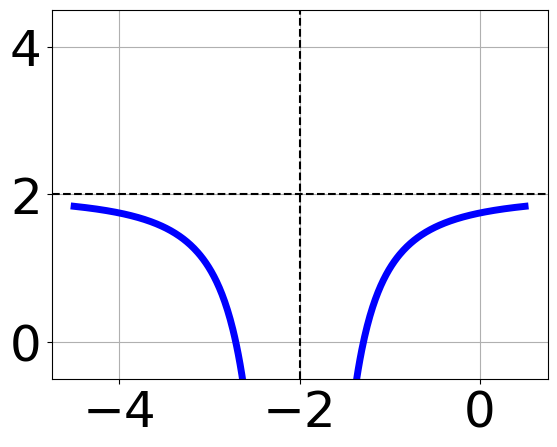
\includegraphics[width = 0.3\textwidth]{../Figures/rationalEquationToGraphCopyAC.png}\item 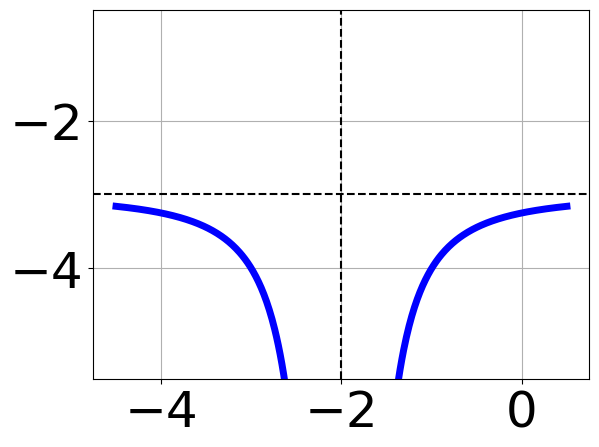
\includegraphics[width = 0.3\textwidth]{../Figures/rationalEquationToGraphCopyBC.png}\item 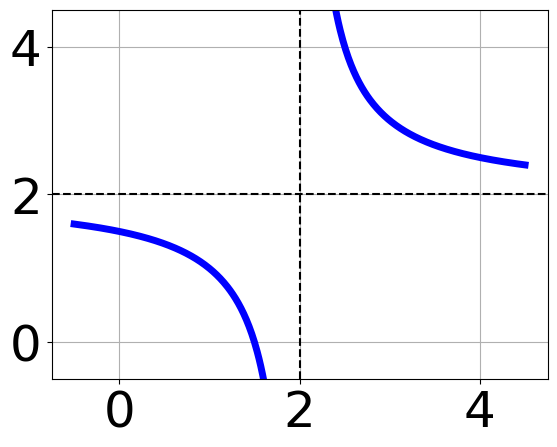
\includegraphics[width = 0.3\textwidth]{../Figures/rationalEquationToGraphCopyCC.png}\item 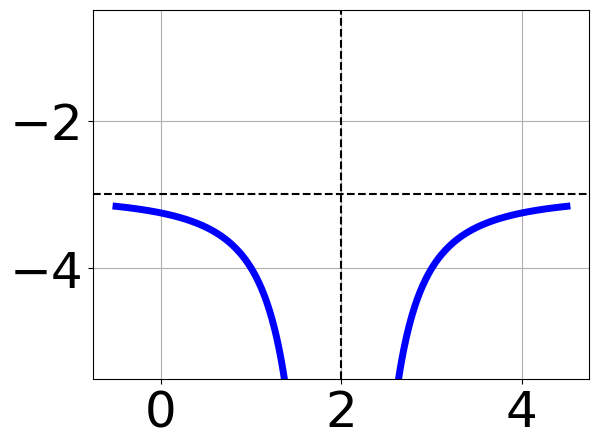
\includegraphics[width = 0.3\textwidth]{../Figures/rationalEquationToGraphCopyDC.png}\end{multicols}\item None of the above.
\end{enumerate} }
\litem{
Determine the domain of the function below.\[ f(x) = \frac{5}{18x^{2} +42 x + 24} \]\begin{enumerate}[label=\Alph*.]
\item \( \text{All Real numbers except } x = a, \text{ where } a \in [-36.1, -35.98] \)
\item \( \text{All Real numbers except } x = a \text{ and } x = b, \text{ where } a \in [-36.1, -35.98] \text{ and } b \in [-12.2, -11.74] \)
\item \( \text{All Real numbers except } x = a, \text{ where } a \in [-1.5, -1.17] \)
\item \( \text{All Real numbers.} \)
\item \( \text{All Real numbers except } x = a \text{ and } x = b, \text{ where } a \in [-1.5, -1.17] \text{ and } b \in [-1.15, -0.86] \)

\end{enumerate} }
\litem{
Choose the equation of the function graphed below.
\begin{center}
    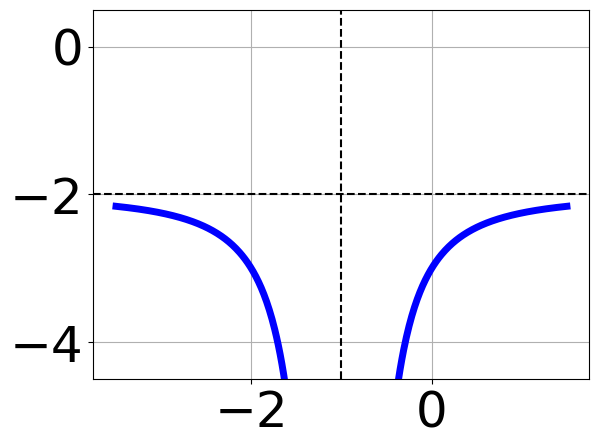
\includegraphics[width=0.5\textwidth]{../Figures/rationalGraphToEquationCopyC.png}
\end{center}
\begin{enumerate}[label=\Alph*.]
\item \( f(x) = \frac{-1}{x + 1} + 1 \)
\item \( f(x) = \frac{-1}{(x + 1)^2} + 1 \)
\item \( f(x) = \frac{1}{x - 1} + 1 \)
\item \( f(x) = \frac{1}{(x - 1)^2} + 1 \)
\item \( \text{None of the above} \)

\end{enumerate} }
\litem{
Choose the equation of the function graphed below.
\begin{center}
    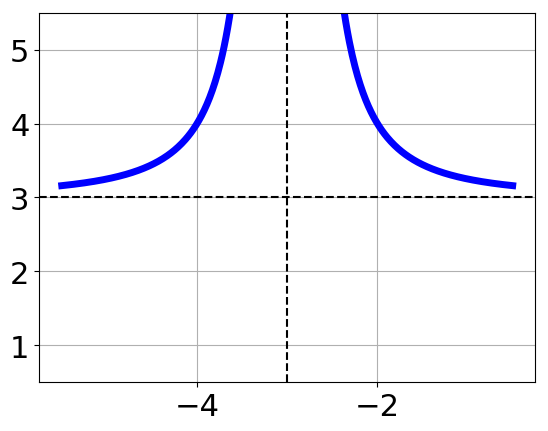
\includegraphics[width=0.5\textwidth]{../Figures/rationalGraphToEquationC.png}
\end{center}
\begin{enumerate}[label=\Alph*.]
\item \( f(x) = \frac{-1}{(x + 3)^2} - 3 \)
\item \( f(x) = \frac{1}{x - 3} - 3 \)
\item \( f(x) = \frac{1}{(x - 3)^2} - 3 \)
\item \( f(x) = \frac{-1}{x + 3} - 3 \)
\item \( \text{None of the above} \)

\end{enumerate} }
\litem{
Choose the graph of the equation below.\[ f(x) = \frac{1}{(x - 1)^2} + 2 \]\begin{enumerate}[label=\Alph*.]
\begin{multicols}{2}\item 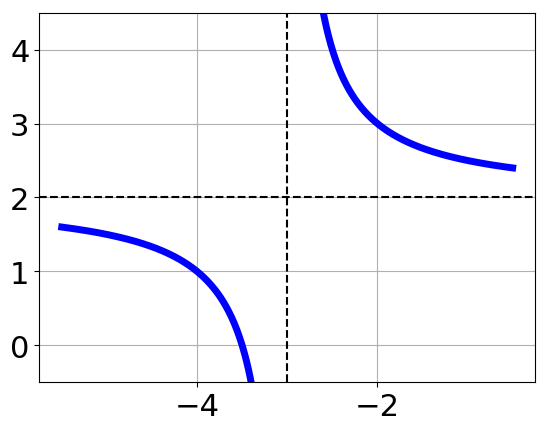
\includegraphics[width = 0.3\textwidth]{../Figures/rationalEquationToGraphAC.png}\item 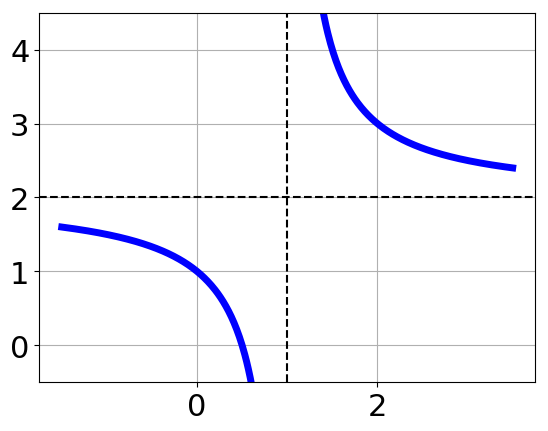
\includegraphics[width = 0.3\textwidth]{../Figures/rationalEquationToGraphBC.png}\item 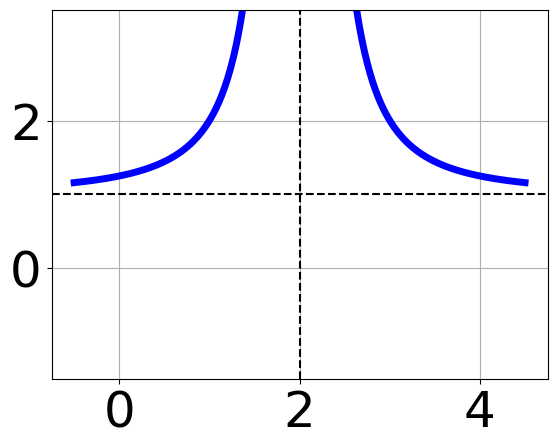
\includegraphics[width = 0.3\textwidth]{../Figures/rationalEquationToGraphCC.png}\item 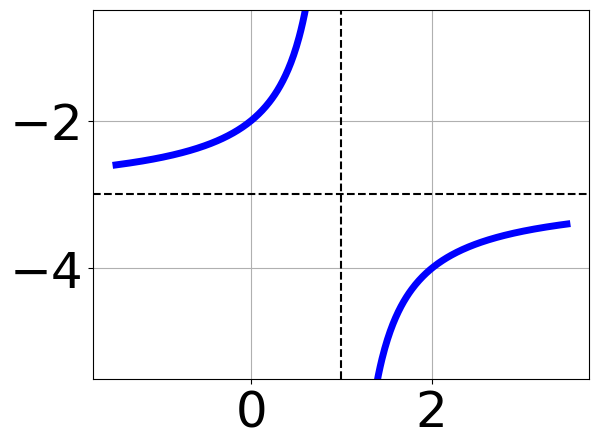
\includegraphics[width = 0.3\textwidth]{../Figures/rationalEquationToGraphDC.png}\end{multicols}\item None of the above.
\end{enumerate} }
\litem{
Solve the rational equation below. Then, choose the interval(s) that the solution(s) belongs to.\[ \frac{-6x}{-5x -3} + \frac{-4x^{2}}{-25x^{2} -5 x + 6} = \frac{4}{5x -2} \]\begin{enumerate}[label=\Alph*.]
\item \( x \in [0.95,2.51] \)
\item \( \text{All solutions lead to invalid or complex values in the equation.} \)
\item \( x \in [-0.23,0.97] \)
\item \( x_1 \in [-0.59, 0.11] \text{ and } x_2 \in [-0.4,3.6] \)
\item \( x_1 \in [-0.59, 0.11] \text{ and } x_2 \in [-1.2,0.2] \)

\end{enumerate} }
\end{enumerate}

\end{document}